\documentclass[a4paper,10pt]{article}
\usepackage[utf8]{inputenc}
\usepackage{amstext}
\usepackage{listings}
\usepackage{graphicx}
\usepackage{subfigure}
\usepackage[T1]{fontenc}
\usepackage[utf8]{inputenc}
\usepackage[font=small,labelfont=bf]{caption}
\usepackage{float}
\usepackage[dutch]{babel}
\usepackage[section]{placeins}

\DeclareCaptionLabelFormat{andtable}{#1~#2  \&  \tablename~\thetable}


%opening
\title{Betrouwbare end-to-end communicatie}
\author{Patrick van Looy \& Bram Leenders}

\begin{document}

\maketitle

\section{Inleiding}
Bij het opzetten van sensornetwerken, kan het zijn dat twee nodes niet in elkaars zendbereik vallen. In een dergelijk geval kan een tussenliggende node helpen door berichten door te sturen. Zo kunnen nodes als schakels in een ketting gebruikt worden om een groter bereik mogelijk te maken.

Een dergelijke constructie is een stuk gecompliceerder dan directe communicatie tussen twee nodes, omdat voor betrouwbare communicatie het zenden van ontvangstbevestigingen nodig is.

\section{Probleemstelling}
Om het probleem overzichtelijk te houden, is het aantal nodes in deze proef beperkt tot drie. Er is een zender, een ontvanger en een doorsturende node. Omdat het aantal nodes beperkt is, is er maar \'e\'en mogelijk pad. Hierdoor kan het pad vooraf vastgelegd worden, dit heet ook wel statische routering.

De uiteindelijke opstelling moet de zender de garantie geven dat een bericht uiteindelijk ontvangen wordt door de ontvanger via de tussenliggende node. 

\section{Protocol}
Om deze garantie te bieden, kan gebruik worden gemaakt van het alternating bit protocol. Dit protocol stuurt een nummer -een bit- mee met een pakket, wanneer de ontvanger het ontvangt stuurt deze bevestiging met datzelfde nummer terug. Indien de zender een bevestiging met het correcte (laatst verzonden) nummer ontvangt, hoogt deze een counter met een op en stuurt deze het volgende pakket.

Figuur~\ref{fig:flow} illustreert het pad dat een pakket met bijbehorende bevestiging aflegt. Figuur~\ref{fig:roles} toont de verschillende staten waarin een zender/repeater/ontvanger zich kan bevinden en de transities tussen deze staten.

\begin{figure}[ht!]
    \centering
    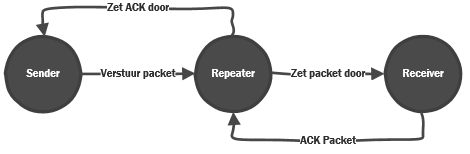
\includegraphics[width=0.8\textwidth]{flow.png}
    \caption{}
    \label{fig:flow}
\end{figure}

\begin{figure}[ht!]
    \begin{minipage}{\textwidth}
        \begin{minipage}{0.49\textwidth}
            \centering
            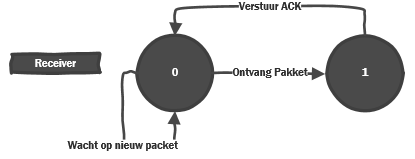
\includegraphics[width=\textwidth]{receiver.png}
            \caption*{Receiver Arduino}
        \end{minipage}
        \hfill
        \begin{minipage}{0.49\textwidth}
            \centering
            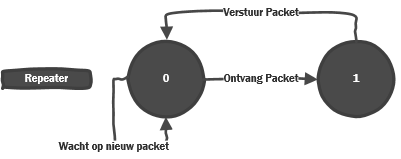
\includegraphics[width=\textwidth]{repeater.png}
            \caption*{Repeater Arduino}
        \end{minipage}
        \hfill\centering
        \begin{minipage}{0.8\textwidth}
            \centering
            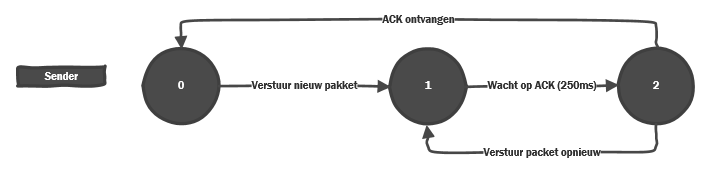
\includegraphics[width=0.95\textwidth]{sender.png}
            \caption*{Sender Arduino}
        \end{minipage}
    \caption{State-diagram Alternating Bit Protocol voor de drie communicerende Arduino's.}
    \label{fig:roles}
    \end{minipage}
\end{figure}

\section{Methodologie}
Onze implementatie gebruikt niet een enkele bit als identificatie van een pakket, maar een getal. Conceptueel verandert dit niets aan het protocol, maar het biedt wel de mogelijkheid voor later uitbreiding. Zo geldt niet langer de restrictie dat er slechts \'e\'en oud pakket in het netwerk mag zitten. Onze implementatie werkt dus ook als oudere berichten (e.g. tien berichten terug) nog ronddolen in het netwerk.

Tevens stuurt de ontvanger een ACK terug die niet de identificatiecode bevat, maar de negatieve waarde hiervan. Hierdoor is het direct duidelijk of een pakket een bevestiging is (indien de code kleiner dan 0 is), of echte data bevat. Dit helpt om ook in grote netwerken ervoor te zorgen dat een zender niet zijn zelf verzonden bericht als ACK kan lezen.

\section{Resultaten}
De implementatie, waarvan de code is bijgevoegd in appendix~\ref{sec:code}, is in verschillende vormen getest:
\begin{itemize}
	\item De zender, repeater en ontvanger allemaal binnen elkaars ontvangstbereik.
	\item De zender en repeater respectievelijk de repeater en ontvanger binnen ontvangstbereik, maar zender en ontvanger buiten ontvangstbereik.
	\item Alleen zender en ontvanger binnen ontvangstbereik; repeater buiten bereik.
\end{itemize}
Omdat er gebruik gemaakt is van statistische routering, is het geen optie voor de zender en ontvanger om direct te communiceren. In de eerste twee gevallen verloopt de communicatie via de repeater; in het derde geval kan geen verbinding worden opgezet omdat de repeater niet bereikbaar is.

\begin{figure}[ht!]
    \begin{minipage}{\textwidth}
        \begin{minipage}{0.3\textwidth}
            \centering
            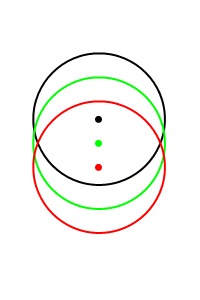
\includegraphics[width=0.9\textwidth]{een.jpg}
            \caption*{Alles bereikbaar}
        \end{minipage}
        \hfill
        \begin{minipage}{0.3\textwidth}
            \centering
            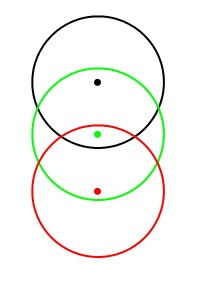
\includegraphics[width=0.9\textwidth]{twee.jpg}
            \caption*{Repeater bereikbaar}
        \end{minipage}
        \hfill
        \begin{minipage}{0.3\textwidth}
            \centering
            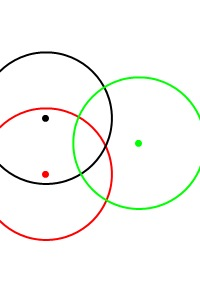
\includegraphics[width=0.9\textwidth]{drie.jpg}
            \caption*{Repeater onbereikbaar}
        \end{minipage}
	\caption{Drie mogelijke scenario's; zwart is de verzender, groen is de repeater en rood is de ontvanger.}
    \end{minipage}
\end{figure}

\section{Conclusie}
Lorem ipsum dolor sit amet, consectetur adipiscing elit. Donec a diam lectus. Sed sit amet ipsum mauris. Maecenas congue ligula ac quam viverra nec consectetur ante hendrerit. Donec et mollis dolor. Praesent et diam eget libero egestas mattis sit amet vitae augue. Nam tincidunt congue enim, ut porta lorem lacinia consectetur. Donec ut libero sed arcu vehicula ultricies a non tortor. Lorem ipsum dolor sit amet, consectetur adipiscing elit. Aenean ut gravida lorem. Ut turpis felis, pulvinar a semper sed, adipiscing id dolor. Pellentesque auctor nisi id magna consequat sagittis. Curabitur dapibus enim sit amet elit pharetra tincidunt feugiat nisl imperdiet. Ut convallis libero in urna ultrices accumsan. Donec sed odio eros. Donec viverra mi quis quam pulvinar at malesuada arcu rhoncus. Cum sociis natoque penatibus et magnis dis parturient montes, nascetur ridiculus mus. In rutrum accumsan ultricies. Mauris vitae nisi at sem facilisis semper ac in est.

Vivamus fermentum semper porta. Nunc diam velit, adipiscing ut tristique vitae, sagittis vel odio. Maecenas convallis ullamcorper ultricies. Curabitur ornare, ligula semper consectetur sagittis, nisi diam iaculis velit, id fringilla sem nunc vel mi. Nam dictum, odio nec pretium volutpat, arcu ante placerat erat, non tristique elit urna et turpis. Quisque mi metus, ornare sit amet fermentum et, tincidunt et orci. Fusce eget orci a orci congue vestibulum. Ut dolor diam, elementum et vestibulum eu, porttitor vel elit. Curabitur venenatis pulvinar tellus gravida ornare. Sed et erat faucibus nunc euismod ultricies ut id justo. Nullam cursus suscipit nisi, et ultrices justo sodales nec. Fusce venenatis facilisis lectus ac semper. Aliquam at massa ipsum. Quisque bibendum purus convallis nulla ultrices ultricies. Nullam aliquam, mi eu aliquam tincidunt, purus velit laoreet tortor, viverra pretium nisi quam vitae mi. Fusce vel volutpat elit. Nam sagittis nisi dui.

Suspendisse lectus leo, consectetur in tempor sit amet, placerat quis neque. Etiam luctus porttitor lorem, sed suscipit est rutrum non. Curabitur lobortis nisl a enim congue semper. Aenean commodo ultrices imperdiet. Vestibulum ut justo vel sapien venenatis tincidunt. Phasellus eget dolor sit amet ipsum dapibus condimentum vitae quis lectus. Aliquam ut massa in turpis dapibus convallis. Praesent elit lacus, vestibulum at malesuada et, ornare et est. Ut augue nunc, sodales ut euismod non, adipiscing vitae orci. Mauris ut placerat justo. Mauris in ultricies enim. Quisque nec est eleifend nulla ultrices egestas quis ut quam. Donec sollicitudin lectus a mauris pulvinar id aliquam urna cursus. Cras quis ligula sem, vel elementum mi. Phasellus non ullamcorper urna.

\newpage
\appendix
\section{Bijlage 1 - Code}
\label{sec:code}
% xxxxxxxxxxxxxxxxxxxxxxxxx Code Snippet STARTS xxxxxxxxxxxxxxxxxxxxxx
\lstset{
  language=C,                     % choose the language of the code
  stepnumber=1,                   % the step between two line-numbers. If it's 1, each line will be numbered
  basicstyle=\footnotesize,
 % numbersep=5pt,                 % how far the line-numbers are from the code
%  backgroundcolor=\color{white}, % choose the background color. You must add \usepackage{color}
  showspaces=false,               % show spaces adding particular underscores
  showstringspaces=false,         % underline spaces within strings
  showtabs=false,                 % show tabs within strings adding particular underscores
  tabsize=4,                      % sets default tabsize to 2 spaces
  captionpos=t,                   % sets the caption-position to top
  breaklines=true,                % sets automatic line breaking
  breakatwhitespace=true,         % sets if automatic breaks should only happen at whitespace
 % title=\lstname,                % show the filename of files included with \lstinputlisting;
 % identifierstyle=\color{identifierColor},
 % caption={Array of Pointers to Strings},
 % frame=lrtb,
 % keywordstyle=\color{purple},         % keyword style
 % commentstyle=\color{blue},           % comment style
 % stringstyle=\color{violet},          % string literal style
 belowcaptionskip = 0.2in,            % Space below caption
 abovecaptionskip = 0.2in             % Space above caption
}
% \lstset{language=C}
\begin{lstlisting}
/*
    Positioning system for Arduino One with RF24 radio chip
*/
#include <SPI.h>
#include "nRF24L01.h"
#include "RF24.h"
#include "printf.h"
#include "MatrixMath.h"

#define N (3)
// Kunstmatige waarde voor Z coordinaten
#define Z 1.0
// Percentage verschil (0 < MAX_DIFF <= 1) dat tussen twee metingen mag zitten.
#define MAX_DIFF (0.25)
// Percentage dat de nieuwste meting in het gemiddelde meetelt (0 < WEIGHT <= 1)
// Bij WEIGHT=1 wordt er geen gemiddelde bijgehouden, maar is de nieuwste meting de enige die meetelt.
#define WEIGHT (0.2)

RF24 radio(3, 9);
unsigned long radiotime;
unsigned long audiotime;
unsigned long timelimit = 50000LL;
uint8_t activeBeacon;

float pos[4][2] = { // Positions van de beacons; pos[1][1] is de y positie van beacon 1
    {0.0, 75.0},
    {72.0, 0.0},
    {294.0, 0.0},
    {372.0, 136.0}
};

float D[4];


void setup() {
  // initialize the serial communication:
  Serial.begin(9600);
  printf_begin();

  // Setup and configure rf radio
  radio.begin();
  radio.setRetries(0,0);

  radio.setDataRate(RF24_2MBPS);
  radio.setChannel(76);
  radio.setPayloadSize(1);
  radio.openReadingPipe(1, 0xdeadbeefa1LL);
  radio.openWritingPipe(0xdeadbeefa1LL);
  radio.startListening();
  radio.setAutoAck(false);
}

void loop() {
  while(radio.available()) { 
    radio.read(&activeBeacon, sizeof(uint8_t)); 
  }
  while (! radio.available());

  radiotime = micros();
  radio.read( &activeBeacon, sizeof(uint8_t));

  if(activeBeacon > 3) { return; }

  while(analogRead(A0) < 50) {
    audiotime = micros();
    if(audiotime - radiotime > timelimit) {
      return; 
    }
  }
  
  float diff = audiotime - radiotime;
  diff = diff * 0.03432; // Afstand tot beacon in cm

  //Zwak uitschieters een beetje af: max 30% increase
  if(diff > (D[activeBeacon]* (1.0 + MAX_DIFF)) && D[activeBeacon] > 0) {
    diff = D[activeBeacon] * (1.0 + MAX_DIFF);
  }
  
  if(diff < (D[activeBeacon]* (1.0 - MAX_DIFF))) {
    diff = D[activeBeacon]*(1.0 - MAX_DIFF);
  }
  
  D[activeBeacon] = D[activeBeacon]*(1.0 - WEIGHT) + diff*WEIGHT; // Weer schuivend gemiddelde */
  //D[activeBeacon] = diff;

  if(activeBeacon == 3) {
    calcPosition();
  }
}

float A[N][N];
float B[N];

void calcPosition() {
    // Relatieve afstanden tussen de nodes; gebruikt node 3 nog niet!
    A[0][0] = 2*pos[1][0] - 2*pos[0][0]; A[0][1] = 2*pos[1][1] - 2*pos[0][1]; A[0][2] = Z;
    A[1][0] = 2*pos[2][0] - 2*pos[1][0]; A[1][1] = 2*pos[2][1] - 2*pos[1][1]; A[1][2] = Z;
    A[2][0] = 2*pos[0][0] - 2*pos[2][0]; A[2][1] = 2*pos[0][1] - 2*pos[2][1]; A[2][2] = Z;
    Matrix.Invert((float*)A,N);

    B[0] = (D[0]*D[0]) - (D[1]*D[1]) - (pos[0][0]*pos[0][0]) + (pos[1][0]*pos[1][0]) - (pos[0][1]*pos[0][1]) + (pos[1][1]*pos[1][1]);
    B[1] = (D[1]*D[1]) - (D[2]*D[2]) - (pos[1][0]*pos[1][0]) + (pos[2][0]*pos[2][0]) - (pos[1][1]*pos[1][1]) + (pos[2][1]*pos[2][1]);
    B[2] = (D[2]*D[2]) - (D[0]*D[0]) - (pos[2][0]*pos[2][0]) + (pos[0][0]*pos[0][0]) - (pos[2][1]*pos[2][1]) + (pos[0][1]*pos[0][1]);
    
    float P3[N];
    Matrix.Multiply((float*)A,(float*)B,N,N,1,(float*)P3);
    printf("Position (P3): (%d,%d)\n", (int) P3[0], (int) P3[1]);
    

    // Relatieve afstanden tussen de nodes; gebruikt node 2 nog niet!
    A[0][0] = 2*pos[1][0] - 2*pos[0][0]; A[0][1] = 2*pos[1][1] - 2*pos[0][1]; A[0][2] = Z;
    A[1][0] = 2*pos[3][0] - 2*pos[1][0]; A[1][1] = 2*pos[3][1] - 2*pos[1][1]; A[1][2] = Z;
    A[2][0] = 2*pos[0][0] - 2*pos[3][0]; A[2][1] = 2*pos[0][1] - 2*pos[3][1]; A[2][2] = Z;
    Matrix.Invert((float*)A,N);

    B[0] = (D[0]*D[0]) - (D[1]*D[1]) - (pos[0][0]*pos[0][0]) + (pos[1][0]*pos[1][0]) - (pos[0][1]*pos[0][1]) + (pos[1][1]*pos[1][1]);
    B[1] = (D[1]*D[1]) - (D[3]*D[3]) - (pos[1][0]*pos[1][0]) + (pos[3][0]*pos[3][0]) - (pos[1][1]*pos[1][1]) + (pos[3][1]*pos[3][1]);
    B[2] = (D[3]*D[3]) - (D[0]*D[0]) - (pos[3][0]*pos[3][0]) + (pos[0][0]*pos[0][0]) - (pos[3][1]*pos[3][1]) + (pos[0][1]*pos[0][1]);
    float P2[N];
    Matrix.Multiply((float*)A,(float*)B,N,N,1,(float*)P2);
    printf("Position (P2): (%d,%d)\n", (int) P2[0], (int) P2[1]);
    
    
    // Relatieve afstanden tussen de nodes; gebruikt node 1 nog niet!
    A[0][0] = 2*pos[2][0] - 2*pos[0][0]; A[0][1] = 2*pos[2][1] - 2*pos[0][1]; A[0][2] = Z;
    A[1][0] = 2*pos[3][0] - 2*pos[2][0]; A[1][1] = 2*pos[3][1] - 2*pos[2][1]; A[1][2] = Z;
    A[2][0] = 2*pos[0][0] - 2*pos[3][0]; A[2][1] = 2*pos[0][1] - 2*pos[3][1]; A[2][2] = Z;
    Matrix.Invert((float*)A,N);
   
    B[0] = (D[0]*D[0]) - (D[2]*D[2]) - (pos[0][0]*pos[0][0]) + (pos[2][0]*pos[2][0]) - (pos[0][1]*pos[0][1]) + (pos[2][1]*pos[2][1]);
    B[1] = (D[2]*D[2]) - (D[3]*D[3]) - (pos[2][0]*pos[2][0]) + (pos[3][0]*pos[3][0]) - (pos[2][1]*pos[2][1]) + (pos[3][1]*pos[3][1]);
    B[2] = (D[3]*D[3]) - (D[0]*D[0]) - (pos[3][0]*pos[3][0]) + (pos[0][0]*pos[0][0]) - (pos[3][1]*pos[3][1]) + (pos[0][1]*pos[0][1]);
    float P1[N];
    Matrix.Multiply((float*)A,(float*)B,N,N,1,(float*)P1);
    printf("Position (P1): (%d,%d)\n", (int) P1[0], (int) P1[1]);
    
    
    // Relatieve afstanden tussen de nodes; gebruikt node 0 nog niet!
    A[0][0] = 2*pos[2][0] - 2*pos[1][0]; A[0][1] = 2*pos[2][1] - 2*pos[1][1]; A[0][2] = Z;
    A[1][0] = 2*pos[3][0] - 2*pos[2][0]; A[1][1] = 2*pos[3][1] - 2*pos[2][1]; A[1][2] = Z;
    A[2][0] = 2*pos[1][0] - 2*pos[3][0]; A[2][1] = 2*pos[1][1] - 2*pos[3][1]; A[2][2] = Z;
    Matrix.Invert((float*)A,N);
   
    B[0] = (D[1]*D[1]) - (D[2]*D[2]) - (pos[1][0]*pos[1][0]) + (pos[2][0]*pos[2][0]) - (pos[1][1]*pos[1][1]) + (pos[2][1]*pos[2][1]);
    B[1] = (D[2]*D[2]) - (D[3]*D[3]) - (pos[2][0]*pos[2][0]) + (pos[3][0]*pos[3][0]) - (pos[2][1]*pos[2][1]) + (pos[3][1]*pos[3][1]);
    B[2] = (D[3]*D[3]) - (D[1]*D[1]) - (pos[3][0]*pos[3][0]) + (pos[1][0]*pos[1][0]) - (pos[3][1]*pos[3][1]) + (pos[1][1]*pos[1][1]);
    float P0[N];
    Matrix.Multiply((float*)A,(float*)B,N,N,1,(float*)P0);
    printf("Position (P0): (%d,%d)\n", (int) P0[0], (int) P0[1]);
    
    // Bereken het gemiddelde van de verschillende metingen:
    int avg[N];
    avg[0] = (int) (P0[0] + P1[0] + P2[0] + P3[0]) / 4.0;
    avg[1] = (int) (P0[1] + P1[1] + P2[1] + P3[1]) / 4.0;
    avg[2] = (int) (P0[2] + P1[2] + P2[2] + P3[2]) / 4.0;
  
    printf("Position: (%d,%d)\n\n", avg[0], avg[1]);
}
\end{lstlisting}

\end{document}
